\subsection*{Question 4.3 - Response to a pitch reference step and comparison with the identified model}

The goal is to compare the pitch response predicted by the model identified in Question 4.2 with the response measured on the drone, for a step in the pitch reference.

\paragraph{Step 1 - Model prediction.}
The model from Question 4.2 is
\begin{equation*}
G(s) = \frac{\Theta(s)}{\Theta_{ref}(s)} = \frac{0.909\,(s + 21.2)}{s^2 + 6.71\, s + 46.5} ,
\end{equation*}
and it was simulated with the reference of the handout, $\theta_{ref}(t) = 0.2$ for $15 \le t < 18$ s and $0$ otherwise (function \texttt{lsim}, script \texttt{sim\_pitch\_step.m}).
The input of $G$ is the pitch command normalized to $[-1, 1]$ and the output is the pitch angle $\theta$ in rad.
The model predicts a rise to a peak of $0.098$ rad at $0.45$ s after the step (an overshoot of $18\%$), followed by a settling at the steady-state value $0.2\,G(0) = 0.083$ rad.

\paragraph{Step 2 - Experiment and processing of the real signal.}
In the experiment the drone hovered first and the reference was applied at $t = 15$ s.
The pitch reference and the pitch were recorded as in Question 4.1 (\texttt{thetaref\_data} and \texttt{theta\_data}, $T_s = 0.03$ s).
The recorded reference (\texttt{thetaref\_data}) is $+0.2$ for $15 \le t < 18$ s and $-0.2$ for $18 \le t < 21$ s, and $0$ afterwards, so only its first step is the one asked in the handout.
Two runs were recorded, and the second one is used because the drone hovered more steadily before the step (standard deviation of $\theta$ of $0.0086$ rad, against $0.019$ rad in the first run).
The real signal is processed as follows.
\begin{itemize}
\item The hover trim is removed, by subtracting the mean of $\theta$ in the $2$ s before the step ($0.010$ rad), so that $\theta$ fluctuates around $0$ before the step, like the model, which starts at rest.
The real $\theta$ before the step is drawn as recorded, and it varies between $-0.018$ and $0.011$ rad in the $2.5$ s before the step.
\item Both signals share the time axis and the sampling ($T_s = 0.03$ s), with $t = 15$ s at the start of the step, and the comparison is done only on the step, $15 \le t \le 17.97$ s ($N = 100$ samples).
After $18$ s the reference is $-0.2$ and the drone is no longer responding to the step, so that part cannot be compared with the model.
\item In Figure~\ref{fig:pitch-step}, after the step the recorded data are drawn only until $\theta$ crosses $0$ rad ($t = 18.22$ s), and the curve is set to $0$ from there on.
This is only a choice of presentation, and the real $\theta$ continued to decrease after the crossing (down to $-0.16$ rad), because of the $-0.2$ reference.
\end{itemize}

\begin{figure}[ht]
\centering
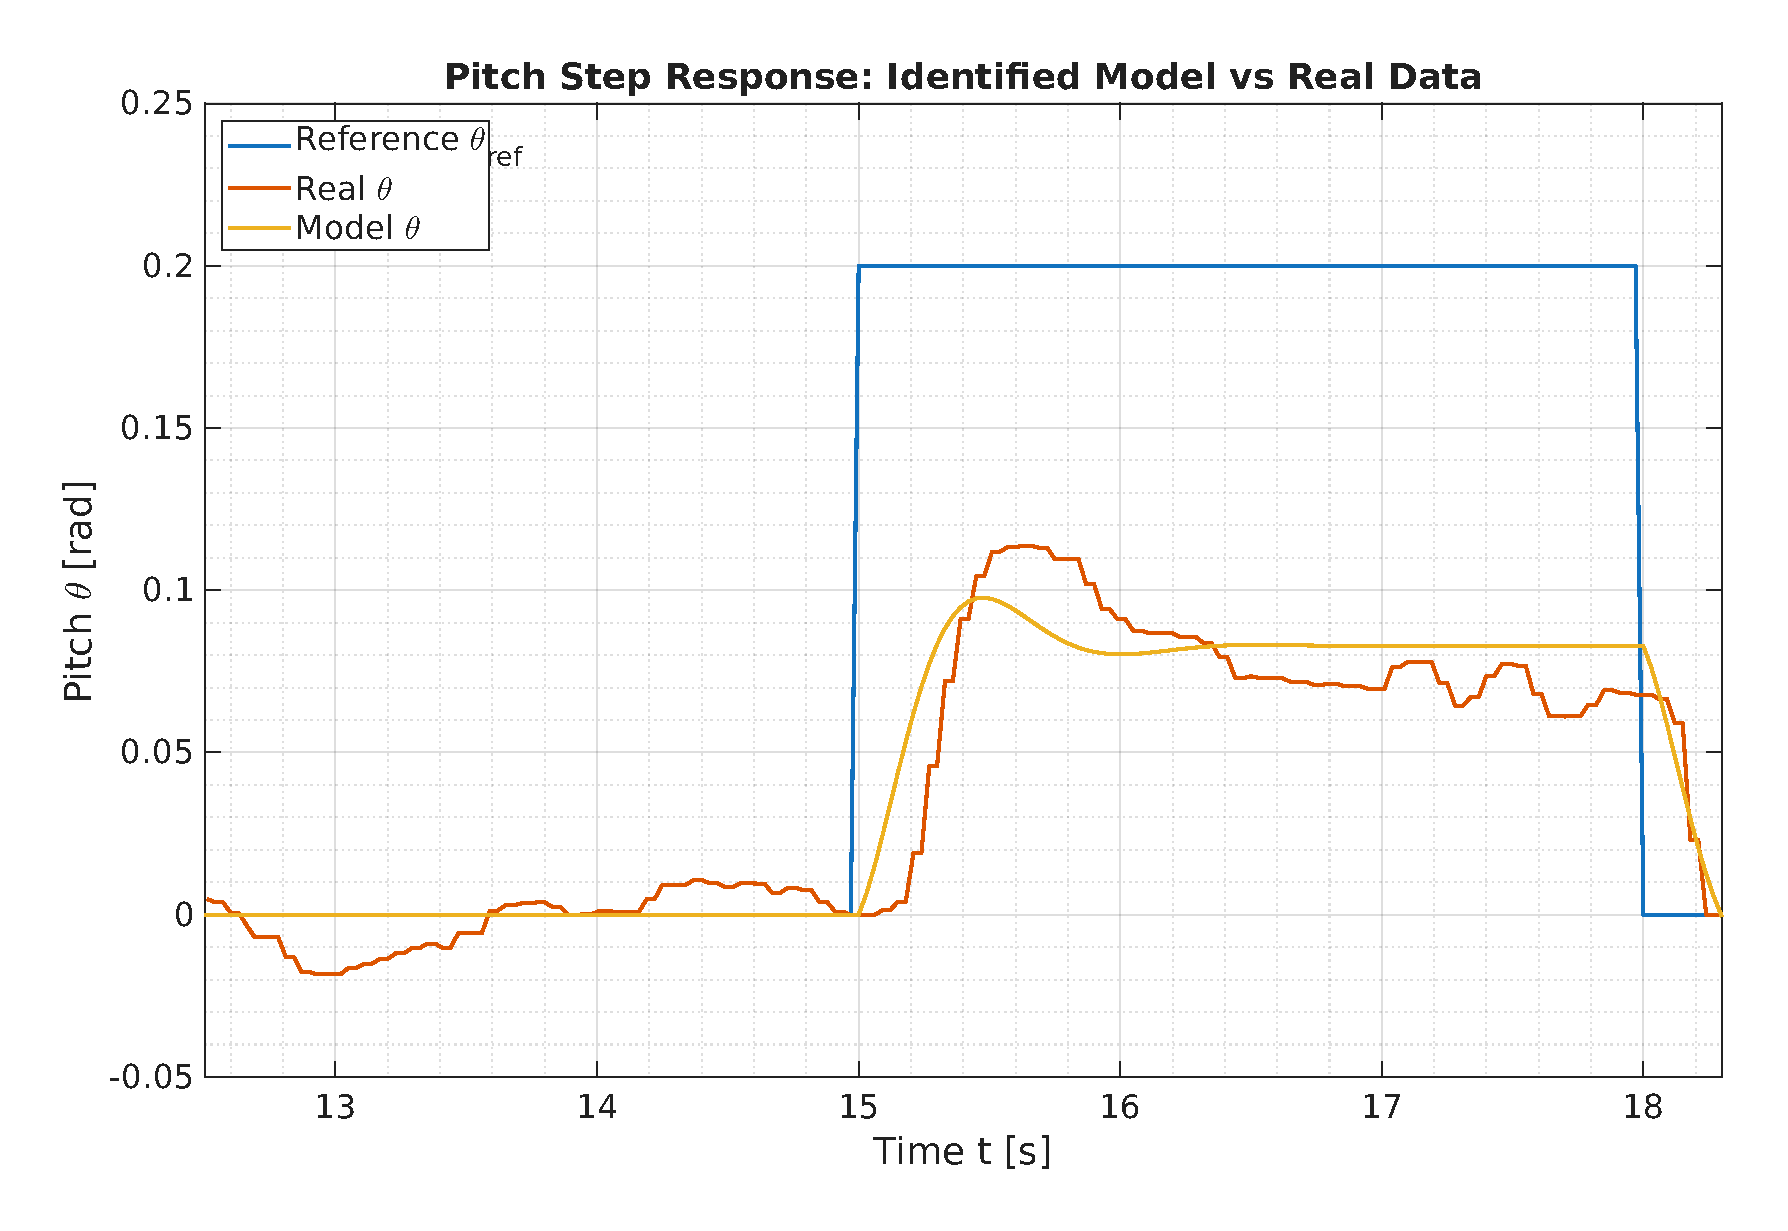
\includegraphics[width=\linewidth]{fig_pitch_step.pdf}
\caption{Pitch response to the reference step: identified model and real data. The real $\theta$ is shown until it crosses $0$ rad after the step and is set to $0$ from there on.}
\label{fig:pitch-step}
\end{figure}

\paragraph{Step 3 - RMSE.}
The model error is measured with the root-mean-square error between the real pitch $\theta_{real}$ and the simulated pitch $\theta_{model}$ on the $N$ samples of the step,
\begin{equation*}
\text{RMSE} = \sqrt{\frac{1}{N} \sum_{k=1}^{N} \big( \theta_{real}(t_k) - \theta_{model}(t_k) \big)^2 } = 0.018 \text{ rad} \approx 1.0^\circ .
\end{equation*}
The RMSE has the unit of $\theta$, which is rad, because both signals are angles.
Its value is $22\%$ of the steady-state pitch predicted by the model ($0.083$ rad), and it is small in absolute terms, about one degree.
Three remarks help to interpret it.
\begin{itemize}
\item \emph{Noise level.} The real $\theta$ fluctuates by about $0.009$ rad (standard deviation) while hovering, so a part of the RMSE is not a model error, since even a perfect model would not reach zero.
\item \emph{Where the error is.} The RMSE is $0.027$ rad in the first second of the step and $0.012$ rad afterwards, so the model is worse in the transient than in the steady state.
\item \emph{Repeatability.} With the first run the RMSE is $0.029$ rad, and the two runs differ from each other by about $0.013$ rad (root-mean-square difference), which is of the same order of the RMSE.
The accuracy of the comparison is therefore limited by the repeatability of the experiment.
\end{itemize}

\paragraph{Step 4 - Discussion.}
\begin{itemize}
\item \emph{Static gain different from $1$.}
The steady-state value of $\theta$ is not equal to the reference: a reference of $0.2$ gives about $0.08$ rad, and $G(0) = K z/\omega_n^2 = 0.414$.
This is not a tracking error.
The input of the system is the pitch command, which is a dimensionless number normalized to $[-1, 1]$, and the output is the angle $\theta$ in rad.
The static gain therefore has the units of rad per unit of normalized command, and it is not the ratio of two quantities of the same kind, so there is no reason for it to be $1$.
Its value is set by how the normalized command is scaled into an angle reference by the drone.
A gain of $1$ would mean that the full command ($1$) gives a pitch of $1$ rad ($57^\circ$), which is not what the drone is meant to do.
The real response confirms this: after the transient, $\theta$ settles at $0.0705$ rad, that is $0.35$ rad per unit of command, close to the $0.414$ of the model and to the gain measured at $1$ rad/s in Question 4.1 ($0.418$).
\item \emph{Level of the steady state.}
The real $\theta$ settles about $15\%$ below the model ($0.0705$ rad against $0.083$ rad).
The static gain of the model comes from the amplitudes measured with sinusoids, and the step may excite amplitude-dependent effects (saturation, dead zone, the onboard controller) that are not in a linear model.
\item \emph{Transient.}
The real response reaches a peak of $0.114$ rad at $0.63$ s, above the $0.098$ rad predicted at $0.45$ s, and then decreases to the plateau.
So the real pitch is less damped than the model, and slower to reach its peak.
Here the model has only the gain of the frequency response as information (Question 4.2), and the magnitude does not fix the phase, or the sign of the zero, which shape the time response.
The step response is thus an independent check of the model, which holds in the order of magnitude and in the overall shape, but not in the details.
\item \emph{Delay.}
The real response reaches $0.05$ rad at $0.33$ s, and the model at $0.18$ s, so the drone is about $0.15$ s late.
This is the delay that was left out of the model in Question 4.2 (Wi-Fi link and onboard processing).
Shifting the model by $0.15$ s decreases the RMSE from $0.018$ rad to $0.012$ rad, so the delay explains about one third of the error.
\end{itemize}

\paragraph{Conclusion.}
The identified second-order model with a zero describes the closed-loop pitch response to the step with an RMSE of $0.018$ rad ($1.0^\circ$) on the step, which is close to the noise level and to the repeatability of the experiment.
The static gain of $0.41$ rad per unit of command is explained by the units of the input and of the output.
The main differences are the delay of about $0.15$ s, the lower steady-state level ($15\%$) and the higher peak of the real response.
A better model would include a delay, for example by multiplying $G(s)$ by $e^{-0.15 s}$ or a Pad\'e approximation of it.
